\section{Como agregar un nuevo algoritmo}
Para agregar un nuevo algoritmo a la aplicaci�n se debe implementar la interfaz \textit{Algorithm}. En la Figura \ref{fig:metaheuristics} se puede ver la interfaz correspondiente.

\begin{figure}[H]
    \centering
    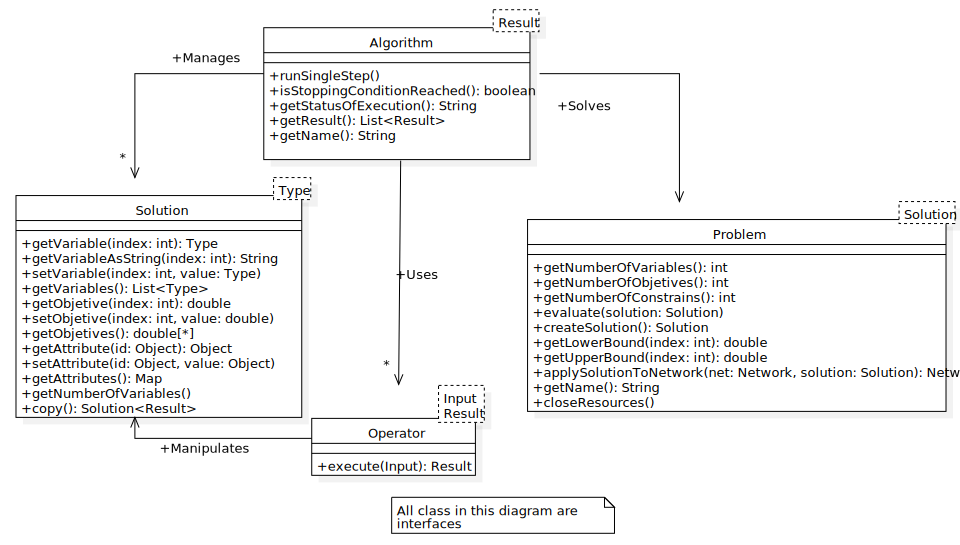
\includegraphics[width=\textwidth]{Seccion1/assets/d_class_metaheuristics}
    \caption{Diagrama de clases del m�dulo de metaheur�sticas.}
    \label{fig:metaheuristics}
\end{figure}

Esta interfaz cuenta con los siguientes m�todos:
\begin{itemize}
    \item \textit{RunSingleStep}: Este m�todo debe ejecutar un �nico paso del algoritmo (Una sola generaci�n/iteraci�n). 
    \item \textit{isStoppingConditionReached}: Este m�todo indica si la condici�n de t�rmino del algoritmo ha sido alcanzada. 
    \item \textit{getStatusOfExecution}: Este m�todo puede devolver un \textit{String} con informaci�n del algoritmo como se muestra en la Figura \ref{fig:getStatusOfExecution} y \ref{fig:getStatusOfExecution2}.
    \item \textit{getResult}: Devuelve el resultado del algoritmo.
    \item \textit{getName}: Devuelve el nombre del algoritmo.
\end{itemize}

\begin{figure}[H]
    \centering
    \includegraphics[width=0.5\textwidth]{Seccion1/assets/SingleObjectiveRunningWindow.png}
    \caption[Mensaje retornado por el m�todo \textit{getStatusOfExecution} en la ventana monoobjetivo.]{Mensaje retornado por el m�todo \textit{getStatusOfExecution} en la ventana monoobjetivo (Est� indicado por la flecha roja).}
    \label{fig:getStatusOfExecution}
\end{figure}

\begin{figure}[H]
    \centering
    \includegraphics[width=0.5\textwidth]{Seccion1/assets/MultiObjectiveRunningWindow.png}
    \caption[Mensaje retornado por el m�todo \textit{getStatusOfExecution} en la ventana multiobjetivo.]{Mensaje retornado por el m�todo \textit{getStatusOfExecution} en la ventana multiobjetivo (Est� indicado por la flecha roja).}
    \label{fig:getStatusOfExecution2}
\end{figure}

Para llevar a cabo la simulaci�n, la aplicaci�n llama al m�todo \textit{RunSingleStep} hasta que \textit{isStoppingConditionReached} sea verdadero. Adicionalmente, dentro del mismo m�todo \textit{RunSingleStep} tambi�n se deber�a asegurar que una vez sea alcanzada la condici�n de termino no se realicen nuevas operaciones. Un ejemplo de \textit{RunSingleStep} utilizado en el Algoritmo NSGAII y GA se puede ver en la Figura \ref{fig:runASingleStep}.
 
\begin{figure}[H]
    \centering
    \includegraphics[width=\textwidth]{Seccion1/assets/runASingleStep.png}
    \caption{M�todo \textit{runASingleStep} para los algoritmos evolutivos.}
    \label{fig:runASingleStep}
\end{figure}

